\documentclass[11pt,a4paper]{scrartcl}
\typearea{12}
\usepackage{graphicx}
\usepackage{pstricks}
\usepackage{listings}
\lstset{language=python}
\pagestyle{headings}
\markright{Computation Neuroscience - Lecture 5}
\begin{document}

\subsection*{Gated channels}

\begin{figure}
\begin{center}
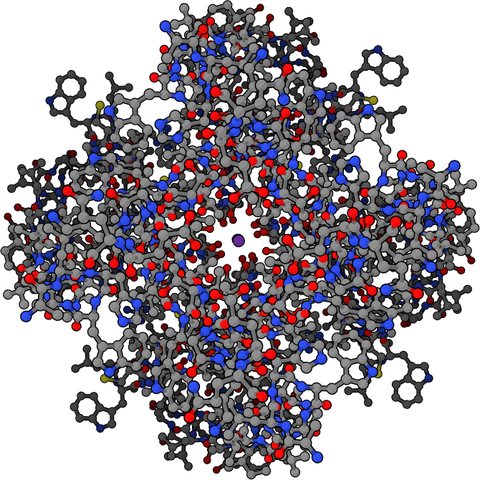
\includegraphics[width=8cm]{potassium_channel.png}
\end{center}
\caption{An open potassium channel, picture from  wikipedia, which in turn took it from the Protein Data Bank. \texttt{http://en.wikipedia.org/wiki/Potassium\_channel}}
\end{figure}

The nonlinear dynamics that neurons rely on to form spikes arise from
the \textbf{voltage-gated channels}; these are ion channels whose
conductance varies as the voltage varies. They are tiny molecular
machines, crucially they are ion selective, only sodium ions can pass
through a sodium gate, only potassium ions through a potassium
gate. Each individual gate has a number of different gating states, we
will briefly examine this, but ultimately each one is either open or
closed, the overall smooth variation, though rapid, variation in these
conductances comes from average a large number of individual discrete
step-like changes as the individual gates open and close.

The potassium channel is a \textbf{persistent} gate; this is actually
a little complicated, but roughly speaking it has one type of closed
state and one type of open state; the sodium channel, which we will
look at after the potassium channel also has one open state, but it
has two types of closed states. 

\begin{figure}
\begin{center}
% GNUPLOT: LaTeX picture with Postscript
\begingroup
  \makeatletter
  \providecommand\color[2][]{%
    \GenericError{(gnuplot) \space\space\space\@spaces}{%
      Package color not loaded in conjunction with
      terminal option `colourtext'%
    }{See the gnuplot documentation for explanation.%
    }{Either use 'blacktext' in gnuplot or load the package
      color.sty in LaTeX.}%
    \renewcommand\color[2][]{}%
  }%
  \providecommand\includegraphics[2][]{%
    \GenericError{(gnuplot) \space\space\space\@spaces}{%
      Package graphicx or graphics not loaded%
    }{See the gnuplot documentation for explanation.%
    }{The gnuplot epslatex terminal needs graphicx.sty or graphics.sty.}%
    \renewcommand\includegraphics[2][]{}%
  }%
  \providecommand\rotatebox[2]{#2}%
  \@ifundefined{ifGPcolor}{%
    \newif\ifGPcolor
    \GPcolorfalse
  }{}%
  \@ifundefined{ifGPblacktext}{%
    \newif\ifGPblacktext
    \GPblacktexttrue
  }{}%
  % define a \g@addto@macro without @ in the name:
  \let\gplgaddtomacro\g@addto@macro
  % define empty templates for all commands taking text:
  \gdef\gplbacktext{}%
  \gdef\gplfronttext{}%
  \makeatother
  \ifGPblacktext
    % no textcolor at all
    \def\colorrgb#1{}%
    \def\colorgray#1{}%
  \else
    % gray or color?
    \ifGPcolor
      \def\colorrgb#1{\color[rgb]{#1}}%
      \def\colorgray#1{\color[gray]{#1}}%
      \expandafter\def\csname LTw\endcsname{\color{white}}%
      \expandafter\def\csname LTb\endcsname{\color{black}}%
      \expandafter\def\csname LTa\endcsname{\color{black}}%
      \expandafter\def\csname LT0\endcsname{\color[rgb]{1,0,0}}%
      \expandafter\def\csname LT1\endcsname{\color[rgb]{0,1,0}}%
      \expandafter\def\csname LT2\endcsname{\color[rgb]{0,0,1}}%
      \expandafter\def\csname LT3\endcsname{\color[rgb]{1,0,1}}%
      \expandafter\def\csname LT4\endcsname{\color[rgb]{0,1,1}}%
      \expandafter\def\csname LT5\endcsname{\color[rgb]{1,1,0}}%
      \expandafter\def\csname LT6\endcsname{\color[rgb]{0,0,0}}%
      \expandafter\def\csname LT7\endcsname{\color[rgb]{1,0.3,0}}%
      \expandafter\def\csname LT8\endcsname{\color[rgb]{0.5,0.5,0.5}}%
    \else
      % gray
      \def\colorrgb#1{\color{black}}%
      \def\colorgray#1{\color[gray]{#1}}%
      \expandafter\def\csname LTw\endcsname{\color{white}}%
      \expandafter\def\csname LTb\endcsname{\color{black}}%
      \expandafter\def\csname LTa\endcsname{\color{black}}%
      \expandafter\def\csname LT0\endcsname{\color{black}}%
      \expandafter\def\csname LT1\endcsname{\color{black}}%
      \expandafter\def\csname LT2\endcsname{\color{black}}%
      \expandafter\def\csname LT3\endcsname{\color{black}}%
      \expandafter\def\csname LT4\endcsname{\color{black}}%
      \expandafter\def\csname LT5\endcsname{\color{black}}%
      \expandafter\def\csname LT6\endcsname{\color{black}}%
      \expandafter\def\csname LT7\endcsname{\color{black}}%
      \expandafter\def\csname LT8\endcsname{\color{black}}%
    \fi
  \fi
  \setlength{\unitlength}{0.0500bp}%
  \begin{picture}(5040.00,3528.00)%
    \gplgaddtomacro\gplbacktext{%
      \csname LTb\endcsname%
      \put(1078,704){\makebox(0,0)[r]{\strut{} 0}}%
      \put(1078,1344){\makebox(0,0)[r]{\strut{} 0.25}}%
      \put(1078,1984){\makebox(0,0)[r]{\strut{} 0.5}}%
      \put(1078,2623){\makebox(0,0)[r]{\strut{} 0.75}}%
      \put(1078,3263){\makebox(0,0)[r]{\strut{} 1}}%
      \put(1210,484){\makebox(0,0){\strut{}-100}}%
      \put(1782,484){\makebox(0,0){\strut{}-80}}%
      \put(2354,484){\makebox(0,0){\strut{}-60}}%
      \put(2927,484){\makebox(0,0){\strut{}-40}}%
      \put(3499,484){\makebox(0,0){\strut{}-20}}%
      \put(4071,484){\makebox(0,0){\strut{} 0}}%
      \put(4643,484){\makebox(0,0){\strut{} 20}}%
      \put(176,1983){\rotatebox{-270}{\makebox(0,0){\strut{}open}}}%
      \put(2926,154){\makebox(0,0){\strut{}$V$}}%
    }%
    \gplgaddtomacro\gplfronttext{%
      \csname LTb\endcsname%
      \put(3656,2203){\makebox(0,0)[r]{\strut{}$n_\infty$}}%
      \csname LTb\endcsname%
      \put(3656,1983){\makebox(0,0)[r]{\strut{}$m_\infty$}}%
      \csname LTb\endcsname%
      \put(3656,1763){\makebox(0,0)[r]{\strut{}$t_\infty$}}%
    }%
    \gplbacktext
    \put(0,0){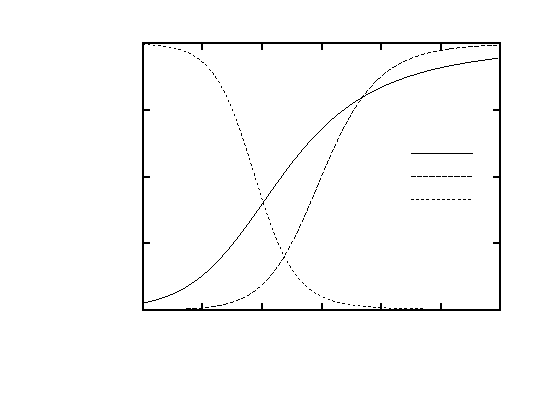
\includegraphics{asymp_vals}}%
    \gplfronttext
  \end{picture}%
\endgroup

\end{center}
\caption{The asymptotic values of the gating probabilities.\label{fig:asymp_vals}}
\end{figure}

The potassium gate is actually composed of four independent subgates,
all these gates must be open to allow potassium ions through, but each
has its own dynamics. The membrane is usually modelled as having
overall potassium conductance 
\begin{equation}
g_{K}=\bar{g}_Kn^4
\end{equation}
where $\bar{g}_K$ would be conductance if all the channels were open
and $n$ is the probability an individual subgate is open so $n^4$ is
the probability an individual gated channel is open. The dynamical equation for $n$ is quite complicated, it is of the standard form
\begin{equation}
\tau_n(V)\frac{dn(t)}{dt}=n_\infty(V)-n(t)
\end{equation}
If $\tau_n(V)$ and $n_\infty(V)$ where constant this would be simple,
$n(t)$ would decay to $n_\infty$ with a timescale of $\tau_n$, however
they aren't constants, they are functions of the membrane potential. 

A graph of $n_\infty(V)$ is shown in Fig.~\ref{fig:asymp_vals}. We can see that $n$ is
small when the voltage is near the resting value but climbs towards
one as $V$ increases. Now, $n$ isn't equal to $n_\infty$, rather it
decays towards it with a time constant given by $\tau_n(V)$, but we
can see that the potassium channels open as the voltage
increases. Before looking at how these play a role in spiking we will
look at the sodium gates. It is worth noting though the way having
four independent gates makes the dynamics crisper: if $n$ is near
zero, $n^4$ even nearer to zero, if $n$ is close to one, $n^4$ is even
closer. 

We also need to discuss reversal potentials. You would expect
the flow of potassium to be determined by $g_KV$, but it isn't; because
there are more potassiums inside the cell than outside they would flow
out even if $V=0$. In fact we assume this doesn't change Ohm's law,
the relationship between potential difference and current, rather, it
just changes the zero point:
\begin{equation}
I_K=g_K(V-E_K)
\end{equation}
where $E_K=-70$ mV, approximately, is called the reversal potential
and can be calculated using an equation called the Nernst equation. In
other words, there is a greater concentration of potassium ions inside
the cell and they are bouncing around with thermal energy, it the
membrane surrounding the cell is conductive to potassium they will
spread out through the membrane. A force is required to keep them in,
the reversal potential is the potential difference needed to reverse
the flow of ions and, we are told, the current-conductivity-potential
relationship is unchanged, except that the potential term $g_KV$ you
would get in a normal circuit is replaced by $g(V-E_K)$.


\begin{figure}
\begin{center}
% GNUPLOT: LaTeX picture with Postscript
\begingroup
  \makeatletter
  \providecommand\color[2][]{%
    \GenericError{(gnuplot) \space\space\space\@spaces}{%
      Package color not loaded in conjunction with
      terminal option `colourtext'%
    }{See the gnuplot documentation for explanation.%
    }{Either use 'blacktext' in gnuplot or load the package
      color.sty in LaTeX.}%
    \renewcommand\color[2][]{}%
  }%
  \providecommand\includegraphics[2][]{%
    \GenericError{(gnuplot) \space\space\space\@spaces}{%
      Package graphicx or graphics not loaded%
    }{See the gnuplot documentation for explanation.%
    }{The gnuplot epslatex terminal needs graphicx.sty or graphics.sty.}%
    \renewcommand\includegraphics[2][]{}%
  }%
  \providecommand\rotatebox[2]{#2}%
  \@ifundefined{ifGPcolor}{%
    \newif\ifGPcolor
    \GPcolorfalse
  }{}%
  \@ifundefined{ifGPblacktext}{%
    \newif\ifGPblacktext
    \GPblacktexttrue
  }{}%
  % define a \g@addto@macro without @ in the name:
  \let\gplgaddtomacro\g@addto@macro
  % define empty templates for all commands taking text:
  \gdef\gplbacktext{}%
  \gdef\gplfronttext{}%
  \makeatother
  \ifGPblacktext
    % no textcolor at all
    \def\colorrgb#1{}%
    \def\colorgray#1{}%
  \else
    % gray or color?
    \ifGPcolor
      \def\colorrgb#1{\color[rgb]{#1}}%
      \def\colorgray#1{\color[gray]{#1}}%
      \expandafter\def\csname LTw\endcsname{\color{white}}%
      \expandafter\def\csname LTb\endcsname{\color{black}}%
      \expandafter\def\csname LTa\endcsname{\color{black}}%
      \expandafter\def\csname LT0\endcsname{\color[rgb]{1,0,0}}%
      \expandafter\def\csname LT1\endcsname{\color[rgb]{0,1,0}}%
      \expandafter\def\csname LT2\endcsname{\color[rgb]{0,0,1}}%
      \expandafter\def\csname LT3\endcsname{\color[rgb]{1,0,1}}%
      \expandafter\def\csname LT4\endcsname{\color[rgb]{0,1,1}}%
      \expandafter\def\csname LT5\endcsname{\color[rgb]{1,1,0}}%
      \expandafter\def\csname LT6\endcsname{\color[rgb]{0,0,0}}%
      \expandafter\def\csname LT7\endcsname{\color[rgb]{1,0.3,0}}%
      \expandafter\def\csname LT8\endcsname{\color[rgb]{0.5,0.5,0.5}}%
    \else
      % gray
      \def\colorrgb#1{\color{black}}%
      \def\colorgray#1{\color[gray]{#1}}%
      \expandafter\def\csname LTw\endcsname{\color{white}}%
      \expandafter\def\csname LTb\endcsname{\color{black}}%
      \expandafter\def\csname LTa\endcsname{\color{black}}%
      \expandafter\def\csname LT0\endcsname{\color{black}}%
      \expandafter\def\csname LT1\endcsname{\color{black}}%
      \expandafter\def\csname LT2\endcsname{\color{black}}%
      \expandafter\def\csname LT3\endcsname{\color{black}}%
      \expandafter\def\csname LT4\endcsname{\color{black}}%
      \expandafter\def\csname LT5\endcsname{\color{black}}%
      \expandafter\def\csname LT6\endcsname{\color{black}}%
      \expandafter\def\csname LT7\endcsname{\color{black}}%
      \expandafter\def\csname LT8\endcsname{\color{black}}%
    \fi
  \fi
  \setlength{\unitlength}{0.0500bp}%
  \begin{picture}(5040.00,3528.00)%
    \gplgaddtomacro\gplbacktext{%
      \csname LTb\endcsname%
      \put(946,704){\makebox(0,0)[r]{\strut{} 0}}%
      \put(946,1344){\makebox(0,0)[r]{\strut{} 2.5}}%
      \put(946,1984){\makebox(0,0)[r]{\strut{} 5}}%
      \put(946,2623){\makebox(0,0)[r]{\strut{} 7.5}}%
      \put(946,3263){\makebox(0,0)[r]{\strut{} 10}}%
      \put(1078,484){\makebox(0,0){\strut{}-100}}%
      \put(1672,484){\makebox(0,0){\strut{}-80}}%
      \put(2266,484){\makebox(0,0){\strut{}-60}}%
      \put(2861,484){\makebox(0,0){\strut{}-40}}%
      \put(3455,484){\makebox(0,0){\strut{}-20}}%
      \put(4049,484){\makebox(0,0){\strut{} 0}}%
      \put(4643,484){\makebox(0,0){\strut{} 20}}%
      \put(176,1983){\rotatebox{-270}{\makebox(0,0){\strut{}time (ms)}}}%
      \put(2860,154){\makebox(0,0){\strut{}$V$}}%
    }%
    \gplgaddtomacro\gplfronttext{%
      \csname LTb\endcsname%
      \put(3656,2203){\makebox(0,0)[r]{\strut{}$\tau_n$}}%
      \csname LTb\endcsname%
      \put(3656,1983){\makebox(0,0)[r]{\strut{}$\tau_m$}}%
      \csname LTb\endcsname%
      \put(3656,1763){\makebox(0,0)[r]{\strut{}$\tau_h$}}%
    }%
    \gplbacktext
    \put(0,0){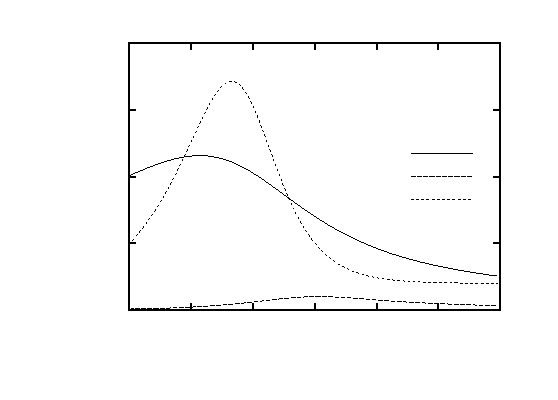
\includegraphics{tau_vals}}%
    \gplfronttext
  \end{picture}%
\endgroup

\end{center}
\caption{The time constants for the gating probabilities.\label{fig:tau_vals}}
\end{figure}


The sodium channel is called a transient channel because it has two
closed states and one open one; generally its dynamics during the
spike is
\begin{equation}
\mbox{closed I}\rightarrow \mbox{open}\rightarrow\mbox{closed II}
\end{equation}
The states are sometimes called \textsl{deactivated} (closed I),
\textsl{activated} (open) and \textsl{inactivated} (closed II).  The
part of the gate that is closed to give the initial closed state is
very like the sodium gate, but with three subgates; the probability of
these subgates being open is usually called $m$; the other part, the
gate that closes to give the second closed state is different in that
it is not made of subgates, its pobability of being open is usually
called $h$ and its asymptotic value, $h_\infty$, is near one for lower
$V$ and near zero for larger. Fig.~\ref{fig:asymp_vals} includes
graphs of $m_\infty(V)$ and $h_\infty(V)$. Finally, the reversal
potential for sodium is $E_{Na}=50$ mV. The sodium current is
therefore
\begin{equation}
I_{Na}=g_{Na}(V-E_{Na})
\end{equation}
with
\begin{equation}
g_{Na}=\bar{g}_{Na}m^3h
\end{equation}

We can now give a rough description of how spikes are formed. The time
constants $\tau$ for the three gating probabilities are given in
Fig.~\ref{fig:tau_values}, these are quite complicated, but the key
thing is that $\tau_m$ is very small, no matter what the value of $V$
is. This means that $m$ stays very close to its asymptotic value
$m_\infty$. As $V$ approaches the threshold of about $-55$ mV, $m$
increases towards one, with $m^3$ increasing even more
dramatically. Opening the sodium gates allows sodium to flood the
cell, increasing the $V$ further and further opening the gates. This
gives the rapid upswing in voltage, the rising part of the spike. The
other two gating probabilities have slower dynamics and it takes $n$
and $h$ a while to catch up with $n_\infty$ and $h_\infty$. However,
as $h$ decreases, it closes the sodium gates again, preventing more
sodium getting in to the cell; $n$ increases opens the potassium
gates, potassium flows out reducing the $V$ again, back towards -70
mV. This gives the downswing of the spike. Afterwards everything
resets.

All of this together gives the Hodgkin-Huxley equation, basically it
equates the rate of change of $V$ to a set of currents, the leak
current giving the roughly linear behavior below threshold we saw in
the integrate and fire model and the gated channels forming the
spike.
\begin{equation}
C_m\frac{dV}{dt}=\mbox{currents}
\end{equation}
For a more accurate model further channels, and therefore further
currents, can be added, other sodium and potassium channels with
different dynamics, or a calcium channel. It is also common to
investigate models \lq{}between\rq{} the integrate and fire model and
the Hodgkin-Huxley equation which add some of the nonlinearity to the
integrate and fire dynamics.

\end{document}

